\documentclass[]{article}
\usepackage{lmodern}
\usepackage{amssymb,amsmath}
\usepackage{ifxetex,ifluatex}
\usepackage{fixltx2e} % provides \textsubscript
\ifnum 0\ifxetex 1\fi\ifluatex 1\fi=0 % if pdftex
  \usepackage[T1]{fontenc}
  \usepackage[utf8]{inputenc}
\else % if luatex or xelatex
  \ifxetex
    \usepackage{mathspec}
  \else
    \usepackage{fontspec}
  \fi
  \defaultfontfeatures{Ligatures=TeX,Scale=MatchLowercase}
\fi
% use upquote if available, for straight quotes in verbatim environments
\IfFileExists{upquote.sty}{\usepackage{upquote}}{}
% use microtype if available
\IfFileExists{microtype.sty}{%
\usepackage{microtype}
\UseMicrotypeSet[protrusion]{basicmath} % disable protrusion for tt fonts
}{}
\usepackage[margin=1in]{geometry}
\usepackage{hyperref}
\hypersetup{unicode=true,
            pdftitle={Machine Learning - Predicting Survival on the Titanic},
            pdfauthor={Sylvia Lee(sylvia19) and Patrick Tung(ptung)},
            pdfborder={0 0 0},
            breaklinks=true}
\urlstyle{same}  % don't use monospace font for urls
\usepackage{longtable,booktabs}
\usepackage{graphicx,grffile}
\makeatletter
\def\maxwidth{\ifdim\Gin@nat@width>\linewidth\linewidth\else\Gin@nat@width\fi}
\def\maxheight{\ifdim\Gin@nat@height>\textheight\textheight\else\Gin@nat@height\fi}
\makeatother
% Scale images if necessary, so that they will not overflow the page
% margins by default, and it is still possible to overwrite the defaults
% using explicit options in \includegraphics[width, height, ...]{}
\setkeys{Gin}{width=\maxwidth,height=\maxheight,keepaspectratio}
\IfFileExists{parskip.sty}{%
\usepackage{parskip}
}{% else
\setlength{\parindent}{0pt}
\setlength{\parskip}{6pt plus 2pt minus 1pt}
}
\setlength{\emergencystretch}{3em}  % prevent overfull lines
\providecommand{\tightlist}{%
  \setlength{\itemsep}{0pt}\setlength{\parskip}{0pt}}
\setcounter{secnumdepth}{0}
% Redefines (sub)paragraphs to behave more like sections
\ifx\paragraph\undefined\else
\let\oldparagraph\paragraph
\renewcommand{\paragraph}[1]{\oldparagraph{#1}\mbox{}}
\fi
\ifx\subparagraph\undefined\else
\let\oldsubparagraph\subparagraph
\renewcommand{\subparagraph}[1]{\oldsubparagraph{#1}\mbox{}}
\fi

%%% Use protect on footnotes to avoid problems with footnotes in titles
\let\rmarkdownfootnote\footnote%
\def\footnote{\protect\rmarkdownfootnote}

%%% Change title format to be more compact
\usepackage{titling}

% Create subtitle command for use in maketitle
\newcommand{\subtitle}[1]{
  \posttitle{
    \begin{center}\large#1\end{center}
    }
}

\setlength{\droptitle}{-2em}

  \title{Machine Learning - Predicting Survival on the Titanic}
    \pretitle{\vspace{\droptitle}\centering\huge}
  \posttitle{\par}
    \author{Sylvia Lee(sylvia19) and Patrick Tung(ptung)}
    \preauthor{\centering\large\emph}
  \postauthor{\par}
      \predate{\centering\large\emph}
  \postdate{\par}
    \date{23 Nov, 2018}


\begin{document}
\maketitle

\subsubsection{Introduction}\label{introduction}

\textbf{Who will survive through the Titanic disaster?}

For most people, ``Titanic'' is both a classic movie and a beautiful
love story. However, the infamous Titanic catastrophe had also been said
to be a prime example of social stratification and status
discriminations in the 1900s. In addition to the ``women and children
first'' evacuation method {[}1{]}, it had been rumored that the lives of
the people with social prestige and high class standing were prioritized
in the momment of danger. In this analysis, we used supervised machine
learning (ML) to answer the question \emph{``What are the 3 strongest
predictors of people who survived on the Titanic?''}

We retrieved the data from
\href{https://www.kaggle.com/c/titanic}{Kaggle's Titanic:Machine
Learning from Disaster} and developed a decision-classification-tree
machine learning model focusing on following features:

\begin{itemize}
\tightlist
\item
  Passenger class
\item
  Sex
\item
  Age
\item
  Number of siblings/spouses onboard
\item
  Number of parents/children onboard
\item
  Fare price
\end{itemize}

In our project, we explored the dataset by generating graphs of the
features' distribution in the population of passengers. Subsequently we
developed the decision tree model using Python's scikit-learn package
and applied the model to a test dataset to predict the survival of the
passenger given the same list of features. Lastly, we summarized our
analysis by calculating the accuracy of our ML model and ranking the
list of features' predictive power.

\subsubsection{Exploratory Analysis}\label{exploratory-analysis}

The RMS Titanic carried enough life boats for only one third of the
passengers, and our data was reflective of this. The data showed
disproportionately larger proportion of passengers that did not survive.
Thus, we compared the feature distributions within the desinated groups,
the ``survived''and the ``did not survive''. We plotted each feature
according to the passenger's survival status (Appendix I). Which allowed
us to gain a sense of the differential distribution of features
depending on the passenger's survival. If all features were equally
weighted dueing evacuation, we assume that the ``survived'' distribution
would have frequecies that equaled to 1/3 of the ``did not survive''.
However, that was not the case.

In general we found the data were reflective of the ``women and children
first'' evacuation policy. There seemed to be larger proportion of women
and children that survived than those that did not. Interestingly, we
found that there were indeed larger proportion of survived passengers
that had the features of ``first class passenger'' and ``paid high fare
price''. On the other hand, family size (number of parent, children,
siblings and spouse) did not appear to cause large difference

\newpage

\subsubsection{Predictions and
Evaluations}\label{predictions-and-evaluations}

\emph{Decision Tree}

We generated a decision classification tree model using scikit-learn
package. In order to reduce overfitting, we ran a 10-folds
cross-validation to find the best \texttt{max-depth} hyperparameter and
developed the learning model accordingly.

In our decision tree model, the first split on the feature ``Sex'',
meaning that the model evaluated gender as the best general feature for
predicting survival. A graphic representation can be found in the
\href{https://github.com/UBC-MDS/sylvia_patrick_Titanic_Survival_ML/blob/master/results/decision_tree.png}{\texttt{results}
repository} folder.

\emph{Predictions}

We ran our trained decision tree model on both the training and testing
dateset to inspect its predictive capabilities (Table 1, Table 2).
Qualitatively inspecting the target (``Survived'') column and the
``Prediction'' column, we found that our model did reasonably well in
the predicting both datasets.

\begin{quote}
\textbf{Table 1.} Snippet of Predictions for both the Training set.
\end{quote}

\begin{longtable}[]{@{}rrrrrrrrr@{}}
\toprule
PassengerId & Pclass & Sex & Age & SibSp & Parch & Fare & Survived &
Prediction\tabularnewline
\midrule
\endhead
1 & 3 & 1 & 22.00000 & 1 & 0 & 7.2500 & 0 & 0\tabularnewline
2 & 1 & 0 & 38.00000 & 1 & 0 & 71.2833 & 1 & 1\tabularnewline
3 & 3 & 0 & 26.00000 & 0 & 0 & 7.9250 & 1 & 0\tabularnewline
4 & 1 & 0 & 35.00000 & 1 & 0 & 53.1000 & 1 & 1\tabularnewline
5 & 3 & 1 & 35.00000 & 0 & 0 & 8.0500 & 0 & 0\tabularnewline
6 & 3 & 1 & 29.69912 & 0 & 0 & 8.4583 & 0 & 0\tabularnewline
7 & 1 & 1 & 54.00000 & 0 & 0 & 51.8625 & 0 & 0\tabularnewline
8 & 3 & 1 & 2.00000 & 3 & 1 & 21.0750 & 0 & 0\tabularnewline
9 & 3 & 0 & 27.00000 & 0 & 2 & 11.1333 & 1 & 1\tabularnewline
10 & 2 & 0 & 14.00000 & 1 & 0 & 30.0708 & 1 & 1\tabularnewline
\bottomrule
\end{longtable}

\begin{quote}
Pclass = Passenger Class, Sex = 0-Female, 1-Male, SibSp =
\#siblings/spouse onboard, Parch = \#parents/children onboard, Survived
= 0-Died, 1-Survived
\end{quote}

\begin{quote}
\textbf{Table 2.}* Snippet of Predictions for Testing set.
\end{quote}

\begin{longtable}[]{@{}rrrrrrrrr@{}}
\toprule
PassengerId & Pclass & Sex & Age & SibSp & Parch & Fare & Survived &
Prediction\tabularnewline
\midrule
\endhead
892 & 3 & 1 & 34.5 & 0 & 0 & 7.8292 & 0 & 0\tabularnewline
893 & 3 & 0 & 47.0 & 1 & 0 & 7.0000 & 1 & 0\tabularnewline
894 & 2 & 1 & 62.0 & 0 & 0 & 9.6875 & 0 & 0\tabularnewline
895 & 3 & 1 & 27.0 & 0 & 0 & 8.6625 & 0 & 0\tabularnewline
896 & 3 & 0 & 22.0 & 1 & 1 & 12.2875 & 1 & 1\tabularnewline
897 & 3 & 1 & 14.0 & 0 & 0 & 9.2250 & 0 & 0\tabularnewline
898 & 3 & 0 & 30.0 & 0 & 0 & 7.6292 & 1 & 1\tabularnewline
899 & 2 & 1 & 26.0 & 1 & 1 & 29.0000 & 0 & 0\tabularnewline
900 & 3 & 0 & 18.0 & 0 & 0 & 7.2292 & 1 & 1\tabularnewline
901 & 3 & 1 & 21.0 & 2 & 0 & 24.1500 & 0 & 0\tabularnewline
\bottomrule
\end{longtable}

\begin{quote}
Pclass = Passenger Class, Sex = 0-Female, 1-Male, SibSp =
\#siblings/spouse onboard, Parch = \#parents/children onboard, Survived
= 0-Died, 1-Survived
\end{quote}

\newpage

\textbf{Model Performance}

To quanititatively evaluate the accuracy of the model, we calculated
both the training and testing accuracies by taking the proportion of
correct predictions In the training and testing datasets (Table 3.). We
then used these accuracy scores. What we were trying to inquire was
whether or not there was an increase in the accuracy of our testing
model in comparison to our training model. This was done to address
possible overfitting problems.

\begin{quote}
\textbf{Table 3.} Prediction accuracy scores of ML model on the training
and testing sets.
\end{quote}

\begin{longtable}[]{@{}lrrrr@{}}
\toprule
Dataset & \#Total Samples & \#Correct predictions & \#Incorrect
predictions & Accuracy Score\tabularnewline
\midrule
\endhead
train & 342 & 266 & 76 & 0.7778\tabularnewline
test & 152 & 128 & 24 & 0.8421\tabularnewline
\bottomrule
\end{longtable}

As you can see, our model predicted the training data set with an
accuracy of 0.7778, predicted the testing data set with an accuracy of
0.8421. Interestingly, we found higher accuracy in our test dataset than
the training dataset, which indicated to us that our model was
adequetely generalizable for data outside of the training model.

\textbf{Feature Importance Ranking}

The ultimate goal of our research was to determine which three variables
features were the most important among others. In order to achieve this
goal, we took our classification tree model and generated an importance
score using the \texttt{sci-kit} learn package. The importance score was
evaluated based on ``gini importance'', which was also known as the
``mean decrease in impurity''. Essentially, the higher the importance
value, the more important that feature was.

\begin{quote}
\textbf{Table 4.} Ranks of each feature based on Gini Importance
\end{quote}

\begin{verbatim}
## Warning in read.table(file = file, header = header, sep = sep, quote =
## quote, : cols = 4 != length(data) = 6
\end{verbatim}

\begin{longtable}[]{@{}rlr@{}}
\toprule
Rank & Feature & Importance\tabularnewline
\midrule
\endhead
1 & Sex & 0.4787907\tabularnewline
2 & Pclass & 0.1702613\tabularnewline
3 & Age & 0.1554545\tabularnewline
4 & Fare & 0.1309192\tabularnewline
5 & SibSp & 0.0496373\tabularnewline
6 & Parch & 0.0149370\tabularnewline
\bottomrule
\end{longtable}

\begin{quote}
Pclass = Passenger Class, SibSp = \#siblings/spouse onboard, Parch =
\#parents/children onboard
\end{quote}

From our results, we determined that the three most important features
in our model were: 1) Sex, 2) Passenger Class, 3) Age. The gini
importances were 0.4788, 0.1703, and 0.1555 respectively.

\subsubsection{Limitations and
Assumptions}\label{limitations-and-assumptions}

First of all, the biggest limitation to our project was that we chose to
explore only one type of model, the decision tree. Given more time and
resources, we could have tested out different models to find the best
predictive model for our problem. However, because we had not yet
learned other ML models, we were wary of conducting an analysis with
unfamiliar methods. In order to compensate for the lack of model
exploration, we used cross validation to pick the best
\texttt{max\_depth} hyperparameter for our decision tree

Cross-validation assumed that all features were iid variables. However,
two of our features might had been correlated. We had \#siblings/spouse
and \#parent/children as two different features, but these two features
could had been analyzed as one feature of ``family size''. Logically,
the two features would have influenced each other, thus undermined the
effectiveness of our cross-validation. However, the high testing
accuracies that we gained at the end of the analysis suggested that this
was not a major problem.

Another limitation that we encountered was that we used means and
medians for the imputation of missing values. As an alternative, we
could use regressors to make predictions on the best value to replace
the missing values. However, this was beyond our current knowledge, so
we resorted to means and medians as sufficient imputation methods for
our predictions.

Lastly, for our prediction, we decided to subset the dataset to only the
relevant features that we were looking for in our research question. The
entire data set that we originally started with had many more features
such as where the passenger embarked, however, to simplify the question
a little bit, we decided to use only a subset of the features to predict
survival rates. Despite using less features, we believe that we still
performed quite well with our predictions.

\subsubsection{Conclusion}\label{conclusion}

We analysed passengers from the RMC Titanic and developed a
classification-tree machine learning model that would allow us to
predict which passenger was more likely to survive based on certain
features. Our machine learning model achieved a fairly high accuracy of
84\% in our testing model. In our analysis, we found that the most
predictive features were gender, passenger class, and age, which cohered
with our expectation that in addition to the ``women and children
first'' evacuation policy, passengers with higher standing were
prioritized as well.

\newpage

\subsubsection{References}\label{references}

Documentation of scikit-learn 0.20.1. (n.d.). Retrieved from

~~~~~~\url{https://scikit-learn.org/stable/documentation.html}

On the importance of the i.i.d. assumption in statistical learning.
(n.d.). Retrieved November 20, 2018, from

~~~~~~\url{https://stats.stackexchange.com/questions/213464/on-the-importance-of-the-i-i-d-assumption-in-statistical-learning}

Titanic: Machine Learning from Disaster. (n.d.). Retrieved November 20,
2018, from

~~~~~~\url{https://www.kaggle.com/c/titanic/data}

Swalin, A. (2018, January 31). How to Handle Missing Data -- Towards
Data Science. Retrieved from

~~~~~~\url{https://towardsdatascience.com/how-to-handle-missing-data-8646b18db0d4}

\newpage

\subsection{Appendix}\label{appendix}

\textbf{Appendix I: EDA Figures}

\emph{Age}

\begin{center}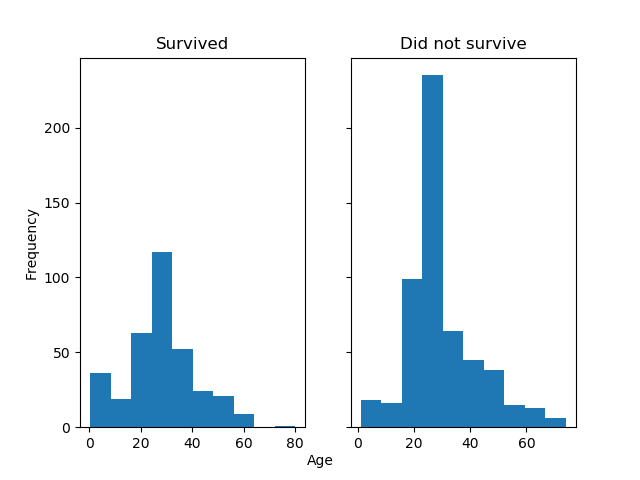
\includegraphics[width=8.89in]{/Users/pokepoke4/Google Drive/UBC MDS - Course Material/Block_3/DSCI_522/sylvia_patrick_Titanic_Survival_ML/results/figure/Age_plot} \end{center}

\begin{quote}
Append 1. Histograms of ages among the passengers that survived (left)
and did not survive (right).
\end{quote}

\newpage

\emph{Sex}

\begin{center}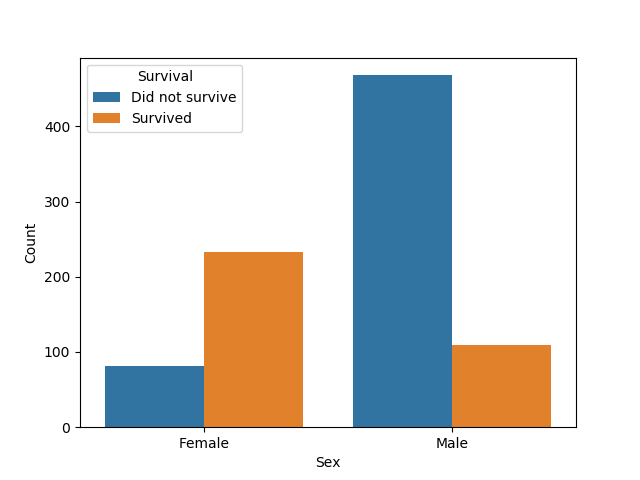
\includegraphics[width=8.89in]{/Users/pokepoke4/Google Drive/UBC MDS - Course Material/Block_3/DSCI_522/sylvia_patrick_Titanic_Survival_ML/results/figure/sex} \end{center}

\begin{quote}
Append 2. Bar plot of sex distribution among the passengers that
survived versus those did not survive.
\end{quote}

\newpage

\emph{Passenger Class}

\begin{center}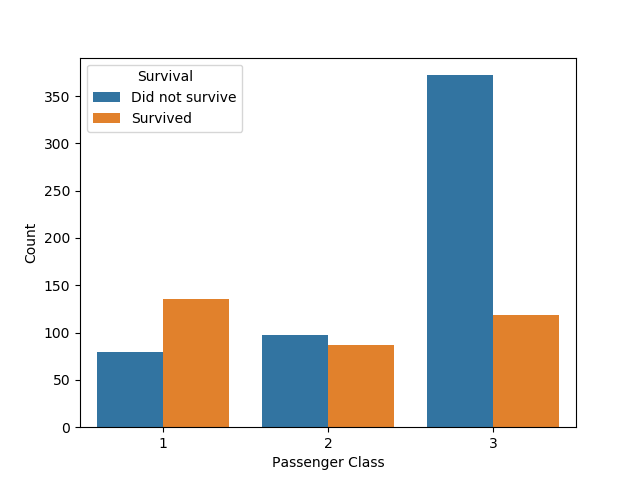
\includegraphics[width=8.89in]{/Users/pokepoke4/Google Drive/UBC MDS - Course Material/Block_3/DSCI_522/sylvia_patrick_Titanic_Survival_ML/results/figure/pclass} \end{center}

\begin{quote}
Append 3. Bar plot of passenger class distribution among the passengers
that survived versus those did not survive.
\end{quote}

\newpage

\emph{Fare Price}

\begin{center}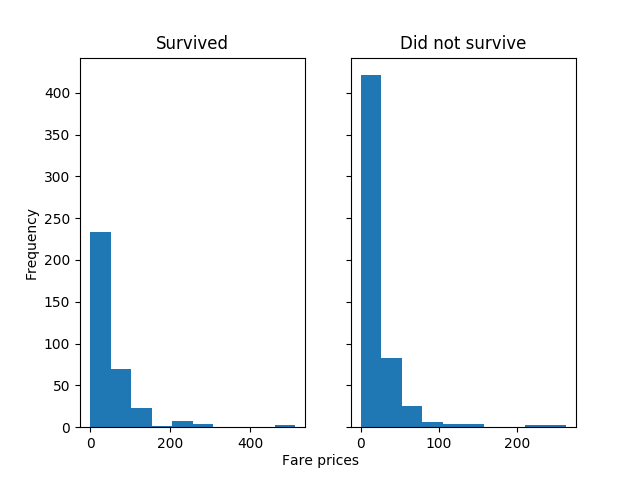
\includegraphics[width=8.89in]{/Users/pokepoke4/Google Drive/UBC MDS - Course Material/Block_3/DSCI_522/sylvia_patrick_Titanic_Survival_ML/results/figure/Fare_plot} \end{center}

\begin{quote}
Append 4. Histograms of fare prices paid by the passengers that survived
(left) and did not survive (right).
\end{quote}

\newpage

\emph{Number of Parents/Children Onboard}

\begin{center}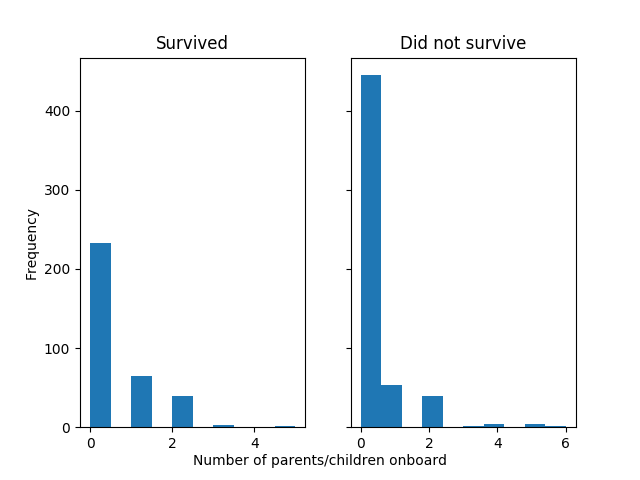
\includegraphics[width=8.89in]{/Users/pokepoke4/Google Drive/UBC MDS - Course Material/Block_3/DSCI_522/sylvia_patrick_Titanic_Survival_ML/results/figure/Parch_plot} \end{center}

\begin{quote}
Append 5. Histograms of number of parent or children that was onboard
with the passengers that did survive (left) and did not survive (right).
\end{quote}

\newpage

\emph{Number of Siblings/Spouses Onboard}

\begin{center}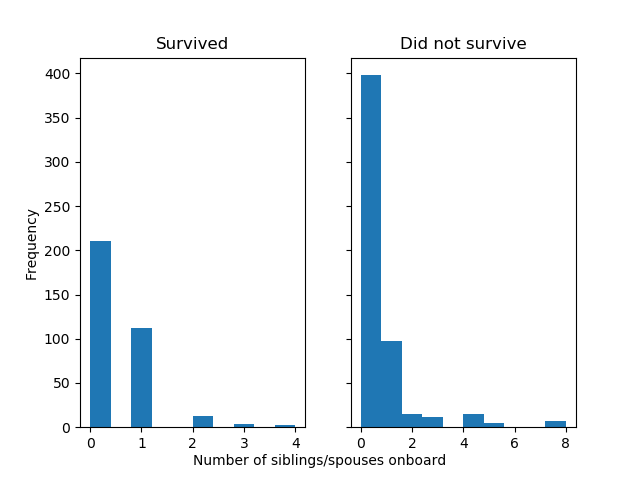
\includegraphics[width=8.89in]{/Users/pokepoke4/Google Drive/UBC MDS - Course Material/Block_3/DSCI_522/sylvia_patrick_Titanic_Survival_ML/results/figure/SibSp_plot} \end{center}

\begin{quote}
Append 6. Histograms of number of siblings or spouse that was onboard
with the passengers that did survive (left) and did not survive (right).
\end{quote}


\end{document}
